\documentclass[tikz,border=5]{standalone}
\usetikzlibrary{fit,positioning,arrows.meta}
\tikzset{neuron/.style={shape=circle, minimum size=1.25cm, 
  inner sep=0, draw, font=\small}, io/.style={neuron, fill=gray!20}}
\begin{document}
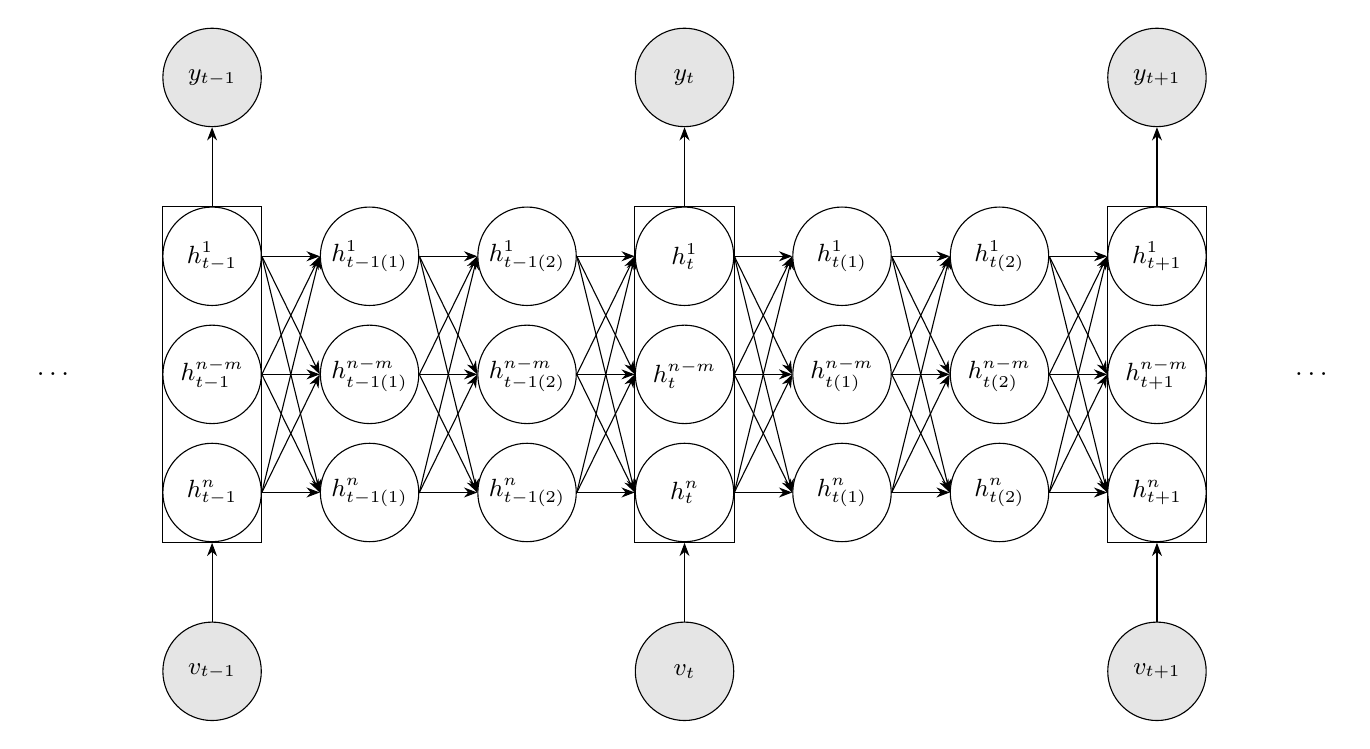
\begin{tikzpicture}[x=2cm, y=1.5cm, >=Stealth]
\foreach \jlabel [count=\j, evaluate={\k=int(mod(\j-1,3)); \jj=int(\j-1);}]
  in {t-1, t-1(1), t-1(2), t, t(1), t(2), t+1}{
    \foreach \ilabel [count=\i] in {1, n-m, n}
        \node [neuron] at (\j, 1-\i) (h-\i-\j){$h_{\jlabel}^{\ilabel}$};
    \ifcase\k
      \node [fit=(h-1-\j) (h-3-\j), inner sep=0, draw] (b-\j) {};
      \node [io, above=of b-\j] (y-\j) {$y_{\jlabel}$};
      \node [io, below=of b-\j] (v-\j) {$v_{\jlabel}$};
      \draw [->] (v-\j) -- (b-\j);
      \draw [->] (b-\j) -- (y-\j);
    \fi
    \ifnum\j>1
      \foreach\i in {1, 2, 3}
        \foreach \ii in {1, 2, 3}
           \draw [->] (h-\i-\jj.east) -- (h-\ii-\j.west);
    \fi
} 
\node [left=of h-2-1] {\ldots};
\node [right=of h-2-7] {\ldots};
\end{tikzpicture}


\begin{tikzpicture}
	\begin{pgfonlayer}{nodelayer}
		\node [style=gn] (0) at (-7, 1) {};
		\node [style=gn] (1) at (-5, 1) {};
		\node [style=gn] (2) at (-3, 1) {};
		\node [style=gn] (3) at (-1, 1) {};
		\node [style=rn] (4) at (-6, -2) {};
		\node [style=rn] (5) at (-4, -2) {};
		\node [style=rn] (6) at (-2, -2) {};
	\end{pgfonlayer}
	\begin{pgfonlayer}{edgelayer}
		\draw [style=arrow] (0) to (4);
		\draw [style=arrow] (0) to (5);
		\draw [style=arrow] (0) to (6);
		\draw [style=arrow] (1) to (4);
		\draw [style=arrow] (1) to (5);
		\draw [style=arrow] (1) to (6);
		\draw [style=arrow] (2) to (4);
		\draw [style=arrow] (3) to (4);
		\draw [style=arrow] (2) to (5);
		\draw [style=arrow] (2) to (6);
		\draw [style=arrow] (3) to (5);
		\draw [style=arrow] (3) to (6);
		\draw [style=arrow, in=45, out=-45, loop] (3) to ();
	\end{pgfonlayer}
\end{tikzpicture}
\end{document}